%! TEX root = **/010-main.tex
% vim: spell spelllang=en:

\subsection{K-NN}%
\label{sub:knn}
\begin{figure}[H]
    \centering
    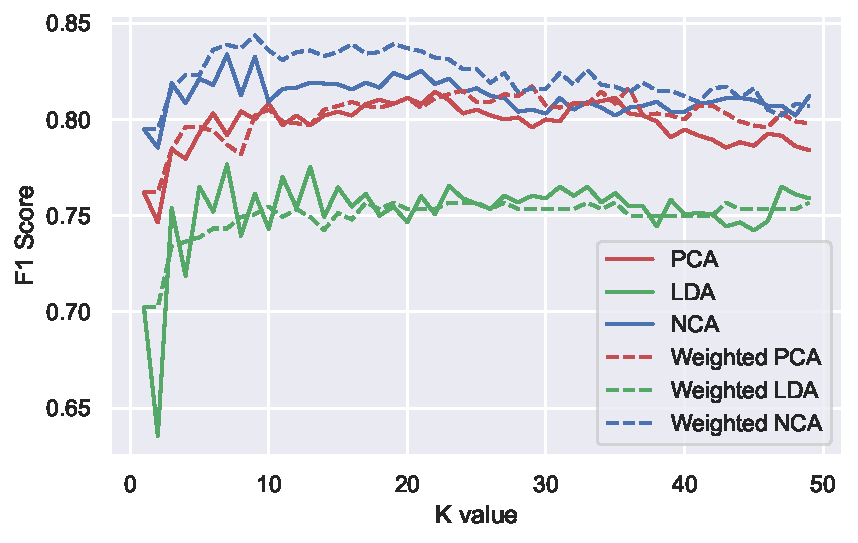
\includegraphics{knn}
    \caption{knn PCA, LDA, NCA}%
    \label{fig:knn_pca_lda_nca}
\end{figure}
% Description of procedure followed for choosing the best k-parameter. Show  a  graph  with  varying  k.  
% Have  you  adjusted  other  parameters  as distance measure? 
% Have you considered removal of irrelevant features if accuracy  is  poor  compared  with  other  approaches?   
% (remember  that  k-nn  is  sensible  to  irrelevant  features  when  computing  distance  to  closest examples
